\section{States, records, and reducers}\label{sec:state}

Part~A, which closed with the catalogue of design patterns in \cref{sec:patterns}, compared
architectures by the decisions each one fixes at design time and the decisions it leaves to the
model at run time. Part~B studies the machinery that carries out those decisions
while a run executes. The machinery has three parts:
\bi
\item \textbf{The state.} The state is the record that the runtime keeps from one step of a run to
the next. This section covers it.
\item \textbf{Routing and termination.} Routing code reads the state to choose the next node or to
stop the run (\cref{sec:control}).
\item \textbf{The tool boundary.} At the tool boundary, the runtime checks a tool call that the
model requested and then executes it (\cref{sec:boundary}).
\ei
The state comes first because the other two parts depend on it. Every step of a run reads and
changes the state, and every routing decision and every limit is a test of one of its fields.

\subsection{The record every node reads and writes}
\label{sec:state-record}

\begin{figure*}[t]
  \centering
  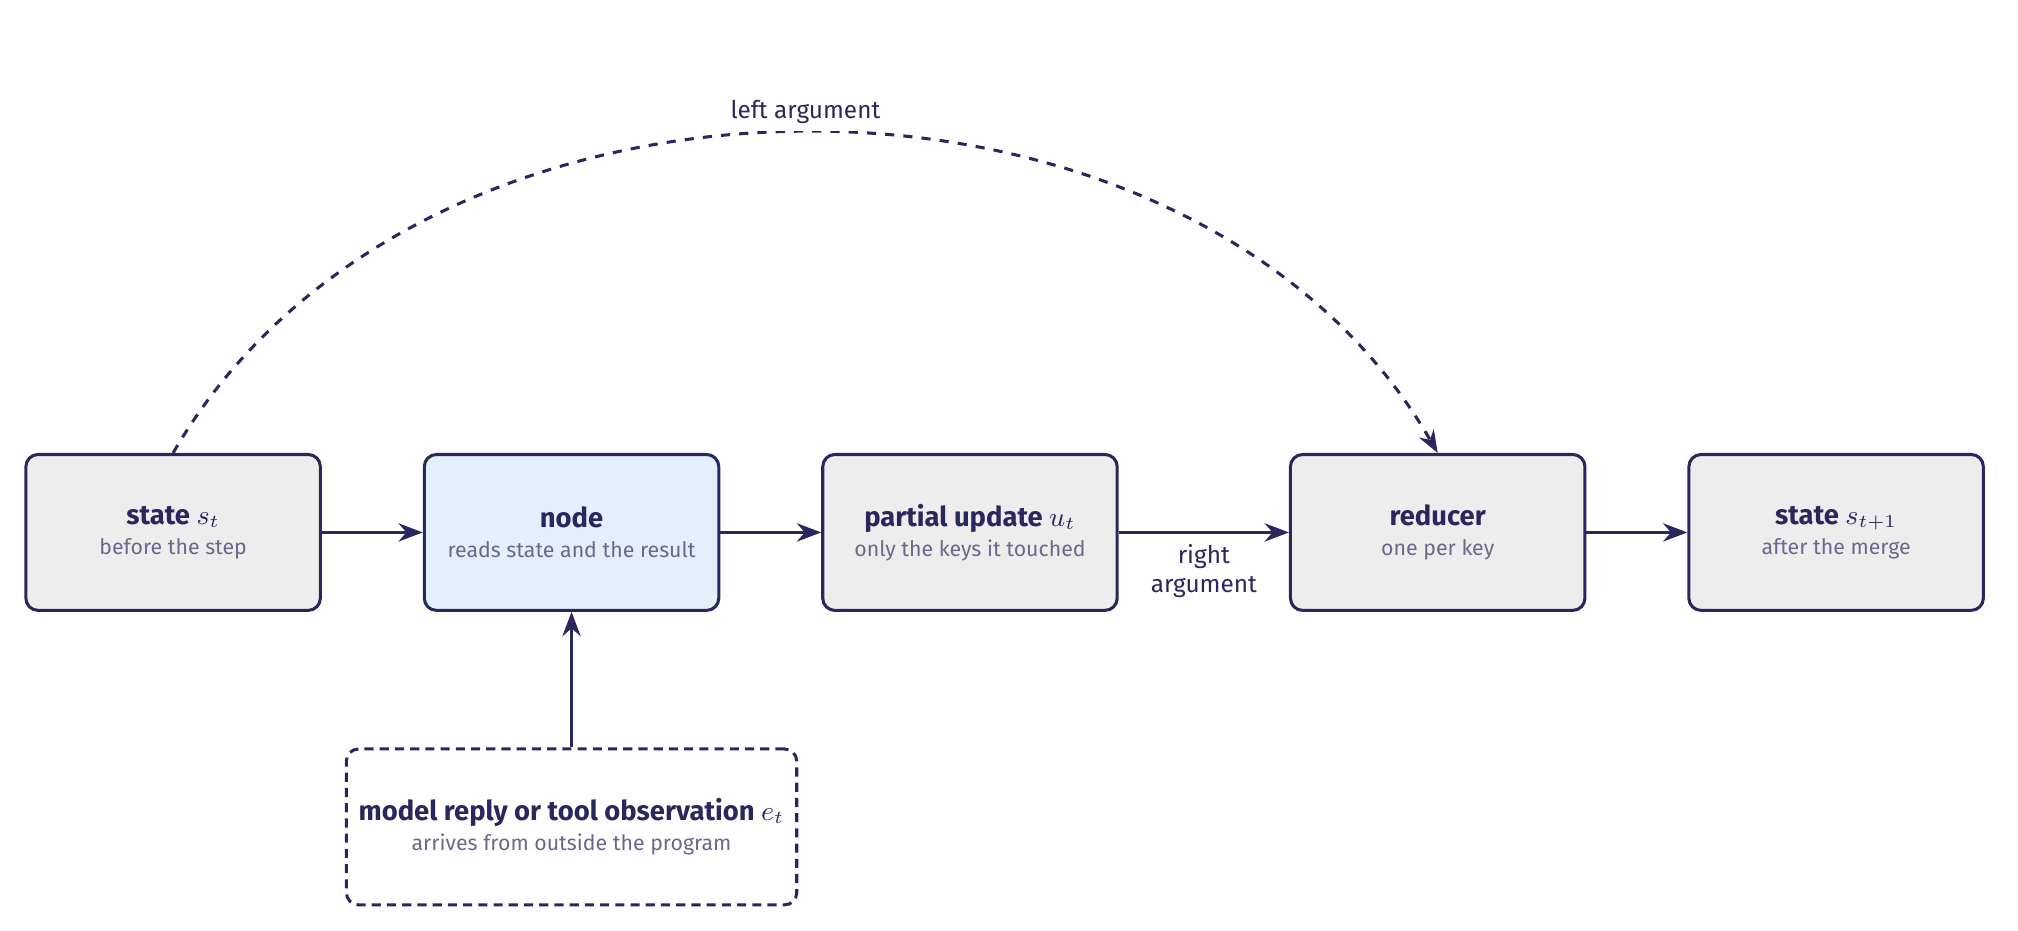
\includegraphics[width=\textwidth]{figures/deck/state-transition.png}
  \caption{One transition. The node reads the state $s_t$ and a result $e_t$ from outside the
  program, a model reply or an observation, and returns a partial update $u_t$. A reducer for each
  field merges the stored value (left argument) with the returned value (right argument) to give
  the state $s_{t+1}$.}
  \label{fig:state-transition}
\end{figure*}

Every node of our agent's graph reads one shared record, the state, and returns a change to it. In
Part~A we drew each version of our agent as a graph. Its nodes are functions that each do the work
of one step: the \demoref{controller} node calls the model, and the \demoref{tools} node executes a
tool call. Its edges say which node may run after which (\cref{sec:reactive}).

The graph shows the order in which nodes may run. It does not show the data they share. In each
version of our agent, that data is a single record.

\begin{definition}[State]
\label{def:state-state}
State is ``a shared data structure that represents the current snapshot of your
application''~\citep{langgraph-graph-api}.
\end{definition}

\Cref{sec:reactive-loop} introduced the state as the record of the run so far. More precisely, the state
is a single data structure that holds what the agent program knows about the run at the current
moment, and every node can read it. It is the record that the vocabulary table
(\cref{tab:agents-vocabulary}) calls the working state.

The word \emph{state} has two other meanings in these notes, and neither is meant here. In
\cref{sec:agents}, the state of the environment included the files of the code base, and the
Controller, Tool and Submit states were the modes of the agent's state machine. The state of this
section belongs to the agent program. It holds what the program has learned about the environment,
such as the file excerpts it has read, while the files themselves stay outside it.

The rest of Part~B relies on the following properties of the state:
\bi
\item \textbf{A declared schema.} The state is declared in advance as a schema, the named set of
fields the state contains, each with a type (\cref{sec:reactive-autonomy}). A \textbf{field}, called a key
in code, is one named entry of the record, such as the list of messages or the number of model
calls made so far (\cref{sec:state-schema}).
\item \textbf{The basis of routing and dispatch.} Routing, which chooses the next node, and
dispatch, which executes a requested tool call, both operate on the state (\cref{sec:control} and
\cref{sec:boundary}).
\ei

The update a node returns is a \textbf{partial update}: it contains only the fields the node
changed and leaves every other field out. In our running example, after a model call the
\demoref{controller} node returns an update that names only \demoref{messages} (the new message),
\demoref{model\_calls} (an increment of one) and \demoref{usage} (the tokens this call used)
(\cref{tab:state-schema}). The runtime adds the increment and the tokens to the stored totals
(\cref{sec:state-reducers}). A node therefore never copies the whole record, and a field that a node
does not mention keeps its value.

\subsection{A transition: propose, then merge}
\label{sec:state-transition}

One step of a run consists of two operations: a node proposes an update, and the runtime merges it
into the state. We call this step a \textbf{transition} of the state, from $s_t$ before the step to
$s_{t+1}$ after it. In \cref{sec:agents}, the same word named a move between two states of the
agent's state machine, such as from Controller to Tool. Here it names one change of the record.
\bi
\item \textbf{Propose.} The node reads $s_t$ together with a result $e_t$ that arrived from outside
the program. This result is either a reply from the model or an observation, the result of one tool
call as the runtime records it (\cref{sec:reactive-loop}). The node returns a partial update $u_t$ that
holds only the fields it changed.
\item \textbf{Merge.} The runtime, the code that executes the graph (\cref{sec:agents-msa}),
combines $u_t$ with $s_t$ to produce $s_{t+1}$. It does this one field at a time.
\ei
In symbols, $u_t = \mathrm{node}(s_t, e_t)$ and $s_{t+1} = \mathrm{merge}(s_t, u_t)$.

\Cref{fig:state-transition} draws one transition. The dashed arc carries the stored value from
$s_t$ to the reducer as its left argument, and the node's partial update enters the reducer as its
right argument. The figure uses \emph{key}, the word for a field in code.

The function that merges one field is that field's \textbf{reducer}.

\begin{definition}[Reducer]
\label{def:state-reducer}
``Each key in the State has its own independent reducer function''~\citep{langgraph-graph-api}.
\end{definition}

A reducer takes two arguments. The left argument is the value already in the state, and the right
argument is the value the node returned. The reducer returns the new value of the field. Every field
that a node can update has its own reducer. A field that is absent from $u_t$ keeps its value from
$s_t$.

We call the node's output a proposal because the node does not decide how it is combined with the
state. Whether a returned list is added to the stored list or replaces it is decided by the field's
reducer, which the runtime applies. The node therefore returns only its own contribution and never
handles the stored value.

The author of a node must still know each field's reducer, because the reducer decides what the
contribution does. For example, an empty list returned for an append field changes nothing
(\cref{sec:state-reset}).

\subsection{Why two runs from one state can diverge}
\label{sec:state-diverge}

The same state can lead to different next states, because each transition also consumes the
external result $e_t$, and the state does not determine that result. There are two reasons:
\bi
\item \textbf{A model reply is sampled.} The model draws its reply from a probability distribution,
so the same input can produce different replies on different calls.
\item \textbf{An observation depends on the files.} The files of the code base are not part of the
state, and the run itself may have edited them. The state alone therefore does not fix what a read
returns.
\ei
Two runs that reach the same state can therefore take different paths after it.

This variation does not make the task environment nondeterministic. In \cref{sec:agents} we
classified our task environment as deterministic: the same read, or the same rescan, on the same
files returns the same result. The model is not part of the environment, which consists of the
working tree at the pinned commit and the alert (\cref{tab:agents-vocabulary}). A sampled reply therefore varies inside the agent and says nothing about
the environment.

A read that returns new content after an edit is still deterministic, because it reads different
files. The term $e_t$ marks the point at which both sources of variation enter a run.

A consequence is that a run can go wrong at a transition even when every node behaves correctly.
The same node, given the same state, can produce a different next state because it received a
different reply, and nothing in the program has misbehaved. Explaining why a run took a particular
path therefore requires the replies and tool results the run actually received, in addition to its
code and its state.

\subsection{Model context, runtime state and durable state}
\label{sec:state-records}

A run keeps several records, which differ in what they hold and in who reads them. Three of them
are defined as follows.
\bi
\item \textbf{Model context} is the input to one model call, which \cref{sec:reactive-loop} called
the model's context. It contains the instructions, the part
of the conversation history selected for this call, and the observations the model needs. The model
reads it.
\item \textbf{Runtime state} is the record that the runtime keeps between steps, which is the state
of this section. It includes fields that never enter a model call. It is read by the nodes, by the
routing functions that choose the next node (also called routers), and by the limits we enforce.
\item \textbf{Durable state} is state written to storage that outlives the process running the
agent. It is read by a run that resumes after its process has stopped.
\ei

\Cref{tab:state-records} summarizes the three records. Compare the last column: each record has a
different reader.

\begin{table}[htbp]
  \caption{Three records of a run: what each one holds and who reads it.}
  \label{tab:state-records}
  \begin{adjustbox}{width=\linewidth}\begin{tabularx}{\linewidth}{@{}L{0.21\linewidth}XL{0.26\linewidth}@{}}
    \toprule
    \textbf{Record} & \textbf{What it holds} & \textbf{Who reads it} \\
    \midrule
    \textbf{Model context} & Instructions, the selected history, and the observations for one call
      & The model \\
    \textbf{Runtime state} & The record kept between steps, including fields that enter no model
      call & Nodes, routers, our limits \\
    \textbf{Durable state} & State written where it survives the end of the process & A resumed
      run \\
    \bottomrule
  \end{tabularx}\end{adjustbox}
\end{table}

Model context and runtime state are easy to confuse, because most of their content overlaps. The
conversation and the tool results, for example, appear in both. Model context is built from runtime
state: before every model call, the runtime assembles the model context from runtime state,
selecting what the call needs. The model's reply then enters runtime state as a new message, through
the \demoref{controller} node's update.

Runtime state also holds fields that serve only to control the run, such as counters. These fields
are never copied into the model context.

Durable state concerns what survives when the process stops. An agent whose state lives only in the
memory of its process cannot resume a run after that process ends. Started again, it knows nothing
of the run. Saving state so that a run can be resumed is the job of components called
checkpointers, which a later unit of the course covers. In these notes, the record carries a run
while it executes. Recovery after a restart is a separate problem.

A fourth record is the trace, the log of events that the runtime writes during a run in the order
they occur (\cref{sec:reactive-edge}). Some of its events come from the \textbf{dispatcher}, the part of
the runtime that checks and executes tool calls. In our agent, the dispatcher does the work of the
\demoref{tools} node (\cref{sec:boundary}). The trace records, for example, each tool request as the
dispatcher received it (\demoref{tool\_request}), each tool result (\demoref{tool\_result}), and
each routing decision.

State and trace answer different questions. The state holds the current value of each field, which
is what the run knows now. The trace holds the sequence of events that led to those values, which
is what the run did. In \cref{sec:control}, we use the trace to follow routing, feedback loops and
termination.

\subsection{Limits the model never sees}
\label{sec:state-counters}

The budget and the stall check, the limits introduced with the reactive loop
(\cref{sec:reactive-stops}), read fields of runtime state that never enter a model call, and we keep
them out of the model context on purpose. In the reactive loop they work as follows:
\bi
\item \textbf{The budget.} The \demoref{controller} node refuses to issue a model call once the
field \demoref{model\_calls}, the number of model calls issued so far, reaches forty.
\item \textbf{The stall check.} The run stops when the last three entries in
\demoref{observations} hold identical results. With a planner, the first such stall leads instead
to one revision of the plan (\cref{sec:planning-stall}). Exactly repeated results are one form in
which a run makes no progress.
\ei

The two thresholds, forty calls and three identical results, never appear in the model context,
and neither does the count in \demoref{model\_calls}. The model does see each tool result, because the
result also reaches it as a message. It never sees the check that compares those results. In the
reactive loop, each limit is a comparison in the code of the \demoref{controller} node, made before
the next model call is issued.

We keep the limits out of the model context so that the model cannot argue with them. A limit
written into the prompt becomes part of the model's input, and the model's response to it is one
more output we cannot predict. The model may follow the limit, or it may produce reasons to continue
past it.

A limit kept in runtime state is a comparison that our code performs. The model's actions still
change the values being compared: each model call adds one to \demoref{model\_calls}, and the
model's tool calls produce the observations. Nothing the model writes, however, can change the
threshold or skip the comparison.

A budget could instead be stated in the \textbf{system prompt}, the instructions placed at the start
of the model context. The two designs differ in the record in which the limit appears. A budget
stated in the system prompt appears in the model context at every call. Our budget is a comparison between the field \demoref{model\_calls} and
the constant forty in the code of the \demoref{controller} node. Neither the field nor the constant
enters the model context.

\subsection{How \texorpdfstring{\msa{}}{mini-swe-agent} represents a state}
\label{sec:state-representations}

Any description of a state, whether of an environment or of an agent's record, can take one of
three forms, which differ in expressive power, meaning how much of the internal make-up of a state
they can describe \citep[\S2.4.7]{russell2020aima}. In order of increasing expressive power:
\bi
\item \textbf{Atomic.} Each state is an indivisible label with no internal parts. Two states can
only be compared as the same or different.
\item \textbf{Factored.} Each state is a fixed set of variables, each with a value. Two states can
agree on some variables and differ on others.
\item \textbf{Structured.} Each state contains objects, each with attributes of its own, and
relationships between those objects.
\ei

\msa{} uses all three, each for a different kind of value.
\bi
\item \textbf{The outcome is atomic.} The outcome of a run, accepted or stopped, is a label with no
internal structure. The score a benchmark reports is a count of such labels, so it records how many
runs succeeded and nothing about how each run got there.
\item \textbf{The record is factored.} The state is a fixed set of named fields with values. Two
states of a run can agree on some fields, such as the alert, and differ on others, such as the
number of model calls.
\item \textbf{The patch and the rejection are structured.} A patch is a set of hunks, the blocks of
changed lines defined in \cref{sec:agents-properties}. Each hunk refers to other objects, a file and a range of
lines in it, so the patch has parts and relationships between them. The rejection, the feedback
returned when a submitted patch fails the checks, is structured in the same way. It refers to the
patch it judged and gives the reasons that patch failed the Submit checks.
\ei

Structure is confined to the patch and the rejection, the two values in which the model's work is
examined: the patch is what the model proposes, and the rejection is the feedback it has to answer.
Everywhere else the record stays factored, because reasoning over structure is harder, both for us
when we write code that reads the state and for the model.

Three mechanisms of Part~B rely on the record being factored, because each one works on a single
named field:
\bi
\item \textbf{Reducers.} Each field can have its own reducer, chosen for that field
(\cref{sec:state-reducers}).
\item \textbf{Routing.} A routing function can test the value of a field, such as
\demoref{status}, instead of interpreting text (\cref{sec:control}).
\item \textbf{Limits.} A limit can be a comparison on a counter field, such as
\demoref{model\_calls}.
\ei

\subsection{The state schema, field by field}
\label{sec:state-schema}

The schema of the state of \msa{} lists the fields of the record, the reducer that merges updates
into each, and what each holds (\cref{tab:state-schema}). The table leaves out the two fields that
the planner uses to detect a stall and to limit revisions, \demoref{failed\_step} and
\demoref{replanned\_at} (\cref{sec:planning-stall}). The column to read first is the reducer, because a field's
reducer decides what later steps can see of that field (\cref{sec:state-reducers}). The rows above
the middle horizontal line are the fields of the reactive loop. The rows below it are the fields
that the planner, the validator and the reflection step add.

\begin{table}[htbp]
  \caption{The state schema of \msa{}. Above the middle line are the fields of the reactive loop;
  below it are the fields that the planner, the validator and the reflection step add.}
  \label{tab:state-schema}
  \begin{adjustbox}{width=\linewidth}\begin{tabularx}{\linewidth}{@{}L{0.29\linewidth}L{0.19\linewidth}X@{}}
    \toprule
    \textbf{Field} & \textbf{Reducer} & \textbf{What it holds} \\
    \midrule
    \demoref{alert}, \demoref{repo}, \demoref{commit}, \demoref{workspace} & none & Set once: the
      alert, the fixture, the pinned commit, the workspace \\
    \demoref{messages} & append & The conversation, in provider form \\
    \demoref{observations} & append & One record per dispatched tool call, refused or not \\
    \demoref{candidate\_patch} & replace & The patch currently proposed \\
    \demoref{model\_calls}, \demoref{usage} & accumulate & Calls issued and tokens spent \\
    \demoref{status} & replace & Running, or the terminal status that ended the run \\
    \midrule
    \demoref{plan} & replace & The subgoals and their status \\
    \demoref{validation} & replace & The latest acceptance decision \\
    \demoref{reflections} & append & Guidance kept from rejected attempts \\
    \demoref{attempt} & explicit & Which attempt is running \\
    \bottomrule
  \end{tabularx}\end{adjustbox}
\end{table}

The fields of the reactive loop fall into four groups:
\bi
\item \textbf{Identity.} \demoref{alert}, \demoref{repo}, \demoref{commit} and \demoref{workspace}
describe the task. \demoref{repo} names the \textbf{fixture}, the code base the agent works on,
which in our running example is OWASP BenchmarkPython at the pinned commit. \demoref{workspace}
names the \textbf{workspace}, the directory that holds the run's working tree, the copy of the
fixture that the run may read and edit (\cref{sec:agents-environment,sec:boundary}). These fields
are set once when the run starts, and no node updates them, so they need no
reducer.
\item \textbf{History.} \demoref{messages} holds the conversation with the model in provider form,
the message format that the model provider's interface expects, so the model context can be built
from it directly. \demoref{observations} holds one observation for every tool call the dispatcher
handled, including the calls it refused to execute, such as a call to a tool that does not exist
(\cref{sec:boundary}).
\item \textbf{Current values.} \demoref{candidate\_patch} holds the patch currently proposed.
\demoref{status} records that the run is still running. Once the run ends, it holds the
\textbf{terminal status} that records why it ended, such as \demoref{accepted} or
\demoref{budget\_exhausted}.
\item \textbf{Counters.} \demoref{model\_calls} counts the model calls issued, and \demoref{usage}
counts the tokens spent.
\ei

The fields below the line belong to the planner, the validator and the reflection step.
\demoref{plan} holds the subgoals and whether each is done (\cref{sec:planning}).
\demoref{validation} holds the latest decision on whether to accept a candidate patch
(\cref{sec:validation}).

The last two fields concern attempts. An \textbf{attempt} is one try at producing an accepted patch.
The \textbf{reflection step} is a node of the complete graph of Part~B (\cref{sec:control}). It runs
after an attempt is rejected and records guidance for the next attempt in \demoref{reflections}. The
field \demoref{attempt} says which attempt is running. No node update is merged into it. It changes
only through an explicit assignment that the runtime makes when a new attempt starts, so the table
marks it \emph{explicit} instead of naming a reducer.

Each of the fields \demoref{plan}, \demoref{validation}, \demoref{reflections} and
\demoref{attempt} enters the schema together with the mechanism that uses it. Adding a mechanism to
the agent is therefore a single change: the mechanism and its fields. The schema never declares a
field for a mechanism that the agent does not have.

\subsection{A TypedDict checks nothing at run time}
\label{sec:state-typeddict}

The schema is declared as a Python \demoref{TypedDict}, a class that lists the keys a dictionary
should have and the type of the value under each key. Its type annotations have two readers, and
neither checks a value while the program runs. A \textbf{type checker}, a program that analyzes source
code without running it and reports values whose types disagree with their declared types, reads
them before the run. LangGraph reads them when the graph is built, but only to find each field's
reducer. Nothing checks a value against its annotation while the agent runs. The declaration looks as follows, with one field shown (\cref{lst:state-typeddict}).

\begin{lstlisting}[basicstyle=\ttfamily\footnotesize, columns=fixed, basewidth=0.525em, keepspaces=true, breaklines=false, xleftmargin=2pt, xrightmargin=2pt, caption={Illustrative code: the state schema declared as a TypedDict, with one field shown.}, label=lst:state-typeddict]
class AgentState(TypedDict, total=False):
    model_calls: Annotated[int, operator.add]
# a model reply puts "forty" here:
# type-checks, and is wrong at run time
\end{lstlisting}

The first line declares the schema as a \demoref{TypedDict}. The argument \demoref{total=False}
makes every field optional, which suits partial updates that name only some fields. The second line
declares \demoref{model\_calls} as an integer, and \demoref{Annotated} attaches
\demoref{operator.add} to it as its reducer, so updates to the field are added to the stored value.
The comment describes the case the declaration does not catch.

At run time, a \demoref{TypedDict} is an ordinary dictionary, and the \demoref{TypedDict} class
itself cannot be used in an \demoref{isinstance} test: \demoref{isinstance(d, AgentState)} raises a
\demoref{TypeError} \citep{pep589}. Suppose a node has a bug that copies a value parsed from
a model reply, the string \texttt{"forty"}, into \demoref{model\_calls}. A value parsed from the
model's text has no declared type, so the type checker accepts the code.

The type checker examined our code before the run, and the value arrived from the model during the
run, so the type checker never saw the value. The code type-checks, and the state is wrong while the
program runs.

Every guarantee about the contents of the state therefore rests on checks written as ordinary code.
A value is checked only where we have written code that checks it. In our agent, the model's
requests enter the run as tool calls, so the check on values that come from the model sits at the
tool boundary, where each tool call is executed (\cref{sec:boundary}).

There, the dispatcher binds the model's arguments to the parameters of the requested tool. Binding
checks the names and the number of the arguments, and it converts a value of the wrong type when the
conversion is unambiguous. It does not check types in general, so it does not reject every wrongly
typed value either.

\subsection{Reducers and what later steps can see}
\label{sec:state-reducers}

A field's reducer decides which of the field's past values later steps can see. The reducer is
chosen per field, and the choice for one field does not affect any other.

Our agent uses three kinds of reducer: append, replace and accumulate. The other two entries in the
reducer column of \cref{tab:state-schema} are not reducers. \emph{None} marks the identity fields,
which no node updates. \emph{Explicit} marks \demoref{attempt}, which only the runtime assigns. The
choice among the three reducers is a choice about visibility, meaning what a later step will be able
to read.
\bi
\item \textbf{Append.} An append reducer adds the new items to the end of the stored list and keeps
all the old ones. \demoref{observations} and \demoref{messages} use it, so they keep the whole
history of the current attempt, and a later step can read every earlier entry.
\item \textbf{Replace.} A replace reducer discards the stored value and keeps the new one.
\demoref{candidate\_patch}, \demoref{plan} and \demoref{status} use it, because each of them states
what is true now: the current patch, the current plan and the current status. A later step sees only
the latest value.
\item \textbf{Accumulate.} An accumulate reducer adds the new numbers to the stored ones.
\demoref{model\_calls} and \demoref{usage} use it, so a later step sees running sums.
\ei

The stall check depends on the append reducer. It compares the last three observations, and only a
field that keeps its history can supply three of them. If \demoref{observations} used a replace
reducer, the state would hold only the latest observation, and the comparison could not be made.

The field \demoref{usage} has two further properties:
\bi
\item \textbf{No running total in a node.} The \demoref{controller} node reports only the tokens
used by the model call it just made, and the reducer adds them to the stored sums. No node computes
or returns the running total, so no node can overwrite it by mistake.
\item \textbf{Separate counters.} The field keeps four token counters, one for each kind of token
the provider reports, and never adds them into a single total. The kinds are not interchangeable.
For example, an input token that the provider processes afresh and an input token that it reads from
its cache of recently processed input are different quantities. A single total could not show
whether cache reads rose while fresh input fell.
\ei

\subsection{Clearing a field that appends}
\label{sec:state-reset}

Returning an empty list does not clear a field whose reducer appends. The problem arises when a new
attempt starts after a rejection. The new attempt is meant to begin without the observations of the
attempt that failed, so that the reasoning that led to the rejected patch does not carry over. A
natural way to write this is for the reflection step to return an empty list for
\demoref{observations} (\cref{lst:state-reset}).

\begin{lstlisting}[basicstyle=\ttfamily\footnotesize, columns=fixed, basewidth=0.525em, keepspaces=true, breaklines=false, xleftmargin=2pt, xrightmargin=2pt, caption={Illustrative code: an attempted reset that leaves the field unchanged.}, label=lst:state-reset]
# the reflection step, starting a new attempt
return {"observations": []}
# merged: every earlier observation is still exactly where it was
\end{lstlisting}

The update does not have the intended effect. The runtime merges it with the field's append
reducer, which adds the items of the returned list to the end of the stored list. Appending an
empty list adds nothing, so the merged value equals the stored value. Every earlier observation
stays in the state, and the new attempt inherits the history it was meant to leave behind.

A plain update cannot clear the field, because an update merged in the usual way passes through the
field's reducer. Clearing it takes an update that bypasses the reducer and assigns the empty list
directly. LangGraph provides this bypass: an update that returns \demoref{Overwrite([])} for the
field replaces the stored list instead of appending to it. In our agent, only the reset step that
starts a new attempt (\cref{sec:control-graph}), which the runtime owns, makes this assignment. Because it changes the state outside the usual merge, the
runtime records it in the trace as a state change, so the reset is visible when the run is
examined.

A reset does not clear every field. Some fields survive it by design:
\bi
\item \textbf{Identity fields} describe the task, which is the same in every attempt.
\item \textbf{Reflections} carry the guidance from rejected attempts into the next attempt, which is
their purpose.
\item \textbf{Counters and \demoref{attempt}} support limits on the run as a whole. If
\demoref{attempt} were reset at the start of each attempt, it would read one in every attempt, so a
limit on the number of attempts could never be reached. If \demoref{model\_calls} were reset, the
budget of forty would bound each attempt instead of the whole run.
\ei

\subsection{One tool result becoming state}
\label{sec:state-tool-result}

Following one tool result into the state shows the mechanisms of this section working together.
Suppose the model has been called once and has asked to read the file the alert names, and the
dispatcher has executed \demoref{read\_file} successfully. At this point \demoref{observations} is
empty, and \demoref{messages} holds the conversation so far. The \demoref{tools} node returns an
update that names two fields (\cref{lst:state-tool-result}).

\begin{lstlisting}[basicstyle=\ttfamily\footnotesize, columns=fixed, basewidth=0.525em, keepspaces=true, breaklines=false, xleftmargin=2pt, xrightmargin=2pt, caption={Illustrative code: the partial update the tools node returns after a successful read.}, label=lst:state-tool-result]
return {"observations": [{"tool": "read_file", "args": {...},
                          "ok": True, "result": "<source>"}],
        "messages": [ToolMessage(...)]}
# merged: one entry appended to each list,
# every other field unchanged
\end{lstlisting}

The update holds one new observation and one new message. The observation records the tool's name,
its arguments, the flag \demoref{ok}, which says whether the call succeeded, and the result. The
\demoref{ToolMessage} is the message that carries the result back to the model in the conversation.

The runtime merges the update field by field. Both fields have append reducers, so each list grows
by one entry. The update names no other field, so every other field, including
\demoref{model\_calls}, keeps its value. The next model context is then assembled from
\demoref{messages} alone. Three properties of the record are visible in this transition:
\bi
\item \textbf{Only the named fields change.} The node named \demoref{observations} and
\demoref{messages}, and no other field of the state changed. A counter advances only when a node returns an update for it.
\item \textbf{The stored observation holds more than the message.} The observation keeps the
arguments and the \demoref{ok} flag alongside the result. The routing functions and the runtime's
accounting, its bookkeeping of what the run has done, read the flag and the arguments directly,
instead of interpreting the text of the message.
\item \textbf{The count stays hidden from the model.} \demoref{model\_calls} was one before the
merge and one after it, and it never appeared in the model's input. This is how the budget remains
a control that the runtime exercises: the model can neither see it nor respond to it.
\ei

After the merge, the state holds the file's content as part of what the run knows. The trace
records the same step as two events, \demoref{tool\_request} and \demoref{tool\_result}, which record
what the run did.

\subsection*{Key points}
\bi
\item The state is a single record declared as a schema of named fields, and in each transition a
node returns a partial update that names only the fields it changed, which the runtime merges field
by field, each field with its own reducer.
\item Two runs can leave the same state along different paths, because model replies are sampled and
tool results depend on files that the run itself may have edited, even though the task environment
is deterministic.
\item Model context is assembled from runtime state for each call, durable state survives the end
of the process, and the trace records what the run did while the state records what it knows now.
\item The state of \msa{} is factored, a fixed set of named fields that reducers, routing and limits
can each read separately, while the patch and the rejection are structured and the outcome of a run
is an atomic label.
\item The budget and the stall check are comparisons in our code, and neither their thresholds nor
the count in \demoref{model\_calls} enter the model context, so the model can neither see the limits
nor argue with them.
\item A \demoref{TypedDict} annotation is not checked at run time, so every guarantee about the
contents of the state rests on checks we write, such as argument binding at the tool boundary, which
itself does not check types in general.
\item A reducer decides what later steps can see (append keeps the history, replace keeps the latest
value, accumulate keeps running sums), so returning an empty list does not clear an append field,
and clearing it takes an assignment that bypasses the reducer (in LangGraph,
\demoref{Overwrite}), which our runtime makes and records in the trace.
\ei
